\documentclass[oneside,11pt,a4paper]{article}

% Chargement d'extensions
\usepackage[utf8]{inputenc}
\usepackage[french]{babel}
\usepackage[T1]{fontenc}
\usepackage{graphicx}
\usepackage[top=3cm, bottom=3cm, left=3cm, right=3cm]{geometry}
% Bout de code
\usepackage{listings}
\usepackage{color}

\definecolor{mygreen}{rgb}{0,0.6,0}
\definecolor{mygray}{rgb}{0.5,0.5,0.5}
\definecolor{mymauve}{rgb}{0.58,0,0.82}

% Commande pour notation 'NB :' (nota bene)
\newcommand\nb[1][0.3]{N\kern-#1emB : }

% csquotes va utiliser la langue définie dans babel
\usepackage[babel=true]{csquotes}

% pour afficher Schéma au lieu de figure dans les legende des images
\addto\captionsfrench{\def\figurename{Schéma}}

% stylisation des enumerations
\frenchbsetup{StandardLists=false} 
\usepackage{enumitem}

% utilisation de lorem lipsum
\usepackage{lipsum}

% Informations le titre, le(s) auteur(s), la date
\title{Hérault Events}
\author{
    Chakib ELHOUITI \and
    Massili KEZZOUL 
}
\date{\today}


\begin{document}
%\maketitle
\begin{titlepage}
	\centering
	{\scshape\LARGE Universite de Montpellier\par}
	{\scshape\Large Rapport de projet Base de données HLIN511\par}
	\vspace{1.5cm}
	{\huge\bfseries Hérault Events\par}
	\vspace{2cm}
	
	{\Large\itshape
		Chakib ELHOUITI : 21813619\\
		Massili KEZZOUL : 21815514\\
		Groupe P \\
		\par}

	\vspace{2cm}
	
	\begin{figure}[h]
		\begin{minipage}[c]{.30\linewidth}
			\centering
			
\includegraphics[width=1\textwidth]{img/um.png}
		\end{minipage}
		\hfill
		\begin{minipage}[c]{.30\linewidth}
			\centering
			
\includegraphics[width=1\textwidth]{img/HE-noir.png}
		\end{minipage}
		\hfill
		\begin{minipage}[c]{.30\linewidth}
			\centering
			
\includegraphics[width=1\textwidth]{img/fds.png}
		\end{minipage}
	\end{figure}

	\vspace{1.5cm}

\vfill
	% Bottom of the page
	{\large \today\par}
\end{titlepage}
\section{Introduction}

Dans le cadre d'un projet commun entre deux UE de la faculté des sciences de l'univérsite de Montpellier, nous avons réaliser une base de données associée à une application web permettant la publication d’événements culturels ou sportifs dans un département donné. Nous avons choisi le département de l'Hérault. L'application peut d'ailleur être visitée à cette adresse `http://webpeda.etu.umontpellier.fr/e20180011096` à condition d'être sur le réseau de l'univérsite de Montepellier.

\section{Modèl entité-association}

\subsection{Schéma E/A}

Tout d'abord nous avons modélisé notre base de données de la manière suivante :

\begin{figure}[h]
  \centering
  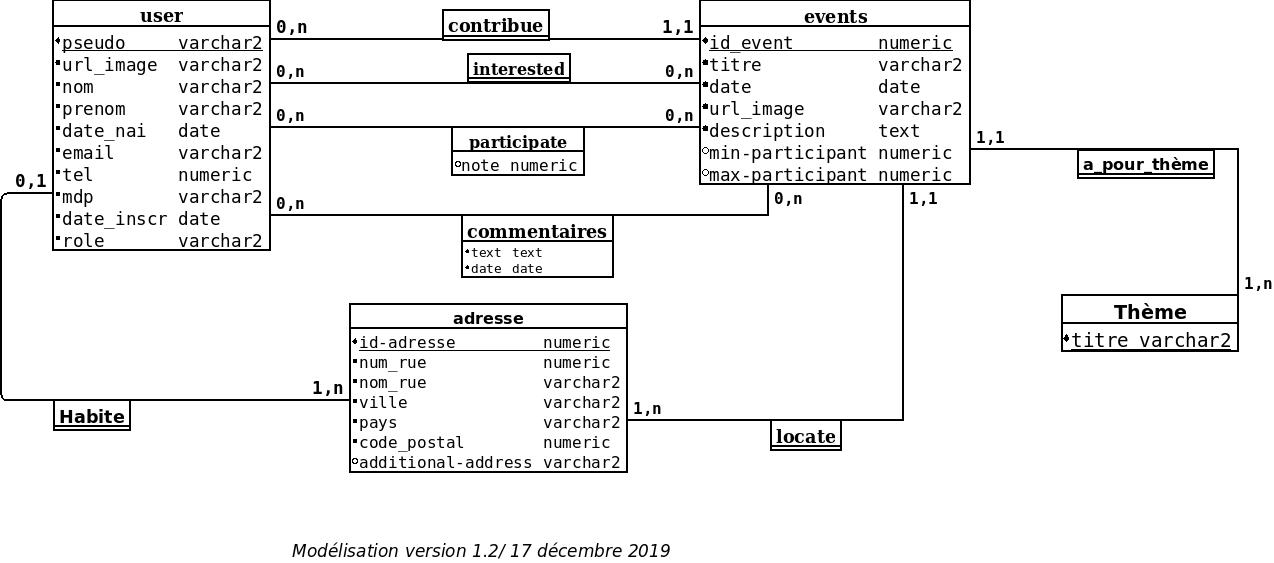
\includegraphics[width=1\textwidth]{img/modelisation.jpeg}
  \caption{Modèl E/A}
\end{figure}

\subsection{Explication du Schéma}

\subsubsection*{Les tables}

\begin{description}
	\item[Adresse :] Cette table permet de stocker l'ensemble des adresses qui seront utilisés par la table \textit{User} et \textit{Events}. On a choisi de ne pas stocker les coordonnées GPS des adresses car ils peuvent être calculés (par une API par example). On a decidé de le faire de cette manière aussi parcequ'il est préferable de ne pas demander des coordonnées GPS à un utilisateur lambda de l'application web.
	\item[User :] La table \textit{User} stock les informations personnelles des utilisateurs du site web. Un utilisateur est identifié par un pseudo qu'il renseigne à son inscription. Ce dernier doit bien évidement être unique.\\ Il existe trois types d'utilisateur : 
	\begin{itemize}[label=\textbullet, font=\small \color{mygray}]
		\item Visiteur ('visitor')
		\item Contributeur ('contributor')
		\item Administrateur ('admin')
	\end{itemize}
	Le type de chaque utilisateur est stocké dans l'attribut \textit{role\_user} qui est une énumération ( de type ENUM ).
	L'attribut \textit{email}, et \textit{tel} doivent être unique.
	\item[Events :] Cette table se charge de stocker les informations relatifs à un événement. Un événement est défini par un identificateur numéric qui générer automatiquement à l'insertion d'un tuple (par AUTO\_INCREMENT) et contient forcément un titre et une date (attribut de type DATETIME). Il peut aussi contenir un lien vers une image (local ou distante), une description (de type TEXT) et un nombre minimum et maximum de participant.
	\item[Theme :] Chaque événement est organisé autour d'un théme donné, donc on a aussi modélisé une table thème afin de stocker tout les thèmes. 
\end{description}

\subsubsection*{Les association}

\begin{description}
	
	\item[Participate : ] cette association permet de stocker les participation des utilisateurs à des évenements.C'est à dire un utlisateur peut participer à plusieurs évenements comme ne pas participer à aucun évenement et un évenement peut avoir aucun ou plusieurs participants. C'est pareil pour les autres associations commentaires et interested
	
	\item[contribuer : ] permet de stocker un utillisateur qui sera un contributeur dans un ou plusieurs évenements. C'est pareil pour les autres associations père/fils. 
	
	
\end{description}

\subsection{Modèle logique de données}
Ensuite nous avons réaliser le modèle relationnel : 
\\	
\textbf{adresse} (\underline{id\_adresse}, num\_rue, nom\_rue, ville, pays, code\_postal, additional\_adresse)\\
\textbf{user}(\underline{pseudo}, nom, prenom, date\_nai, email, tel, mdp, date\_inscr, role, \textit{id\_adresse})\\
\textbf{events}(\underline{id\_event}, titre, date, url\_image, description, min-participant, max-participant, \textit{pseudo\_contributeur}, \textit{id\_adresse}, \textit{theme})\\
\textbf{thème}(\underline{titre})\\
\textbf{particiapte}(\underline{\textit{pseudo}, \textit{id\_event}}, note)\\
\textbf{interested}(\underline{\textit{pseudo}, \textit{id\_event}})\\
\textbf{commentaires}(\underline{\textit{pseudo}, \textit{id\_event}}, text, date).\\

\subsection{Traduction du modèle relationnel en Langage sql (Définition des données)}
Enfin on a écrit le script sql permettant de créer les tables du modèle relationnel (MYSQL).
\section{Les procédures}
\begin{description}
	\item[ throw\_err : ] C'est une procédure qui jette une erreur et affiche  un message donné en paramètres, elle est utilisé dans les triggers et les procédures pour les arrêtées avec une erreur.
	 
	\item[events\_users\_par\_annee] C'est une Procédure, elle prend en paramètres une année et une chaîne de caractères(events ou utilisateurs),si le deuxième paramètres est events, la procédure affiche les évenements de l'année donnée en paramètres, si non elle affiche les utilisateurs inscrit pendant l'année donnée en arguments.
	\item[events\_par\_commentaires : ] C'est une Procédure, elle prend en paramètres une chaîne de caractères (asc ou desc pour l'ordre), elle ordonne les évenements par nombre de commentaires soit par ordre croissant ou décroissant selon la chaîne donnée en paramètres.
\end{description}
\section{Les fonctions}
\begin{description}
	
	\item[note\_event : ] C'est une fonction, elle prend en paramètres un id\_event(un évenement) et calcul sa note moyenne.
	
	\item[nb\_participate : ] C'est une fonction, elle prend en paramètres un id\_event(un évenement) et calcul le nombre de particpants à cet évenement.
	
	\item[nb\_interesses : ] C'est une fonction, elle prend en paramètres un id\_event(un évenement) et calcul le nombre d'intéressés à cet évenement.
	\item[classement\_event : ] C'est une fonction, elle prend en paramètres un id\_event(un évenement) et retourne le classement de l'évenemets par note moyenne, c'est à dire son classement parmi tous les évenements, s'il y'a des évenements de même note, la fonction retourne son classement par note et par son id(du plus petit au plus grand).
	
	
\end{description}
\section{Les triggers}

On aussi créer quelques triggers, qui s'éxecute lors des insertions de tuples, afin d'empêcher d'inserer des tuples qui risque de génerer des incohérences de données (BEFORE) ou bien d'éxecuter des actions (AFTER).

\begin{description}
	\item[BEFORE\_INSERT\_USER : ] Ce trigger vérifie qu'un utilisateur à plus de 12 avant de l'inserer (Respectivement 'BEFORE\_UPDATE\_CONTRIBUTEUR\_EVENT' lors de la mise à jour), il calcul la difference entre la date d'aujourd'hui et la date de naissance donnée. si l'utilisateur a moin de 12 ans alors une erreur est géneré (Erreur 45000).
	\item[BEFORE\_INSERT\_CONTRIBUTEUR\_EVENT : ] Ce trigger vérifie, lors de l'insertion d'un événement (Respectivement 'BEFORE\_UPDATE\_CONTRIBUTEUR\_EVENT' lors de la mise à jour), que le contributeur n'a pas comme rôle 'visitor'. Ce derniér ne peuvent pas contribuer.
	\item[BEFORE\_INSERT\_DATE\_EVENT : ] Ce trigger vérifie à l'inserion d'un événement (Respectivement 'BEFORE\_UPDATE\_DATE\_EVENT' lors de la mise à jour) que la date de ce dernier est supérieur à la date d'aujourd'hui. Il est impossible d'inserer un événement qui est déjà passé.
	\item[BEFORE\_INSERT\_NOTE\_PARTICIPATE : ] Ce trigger empeche d'inserer de note dans la table \textit{participate} tant que l'evenement n'est pas encore passé.
	\item[AFTER\_INSERT\_PARTICIPATE\_INTERESTED : ] Lorsqu'un utilisateur participe à un événement il est considéré comme étant intéressé par cette événement. Ce trigger insére donc l'utilisateur dans la tables \textit{interested} (si il n'y est pas déjà) après son insertion dans la table \textit{participate}.
\end{description}

\section{Conclusion}

\subsection{Les problèmes recontrés}
On a rencontré quelques problèmes concernant la syntaxe mysql, qui était un peu difficile pour créer des triggers et des procédures, aussi 

\subsection{Les compètences acquises}

Pour conclure, à l’issue de ce projet nous avons réussi à réaliser un site web fonctionnel et prèt à l'utilisation. 

Ce projet nous aura permis d’aprofondir nos connaissances en développement web et de compléter nos acquis sur les outils de base du web, tel que :HTML, CSS, PHP et JAVASCRIPT.

\end{document}
